\documentclass[english]{article}
%%%%%%%%%%%%%%%%%%%%%%%%%%%%%%%%%%%%%%%%%%%%%%%%%%%%%%%%%%%%%%%%%%%%%%%%%%%%%%%%%%%%%%%%%%%%%%%%%%%%%%%%%%%%%%%%%%%%%%%%%%%%
\usepackage{latexsym,amsmath,amssymb,amsfonts,fullpage,graphicx, float}


\begin{document}
Gabrielle Merritt
\begin{center}
{\textbf{MEAM 620 Homework 2}} \\
Due: February 18, 2015, 11:59pm
\end{center}


\paragraph{1.} List two advantages and two disadvantages each for using (a) rotation matrices;(b) axis angle representation; (c) exponential coordinates; (d) Euler angles; and (e) quaternions to describe rotations? 
\paragraph{Solution}
a)  Rotation matrices are easy to conceptualize, and can simply multiply rotation matrices to produce another rotation. Some difficulties with Rotation matrix representation is that you cannot represent all orientations without hitting singularities. Additionally rotation matrices need 9 numbers to represent an orientation  compared to the four needed for  axis angle and quaternion. 
\linebreak
b) Axis angle representation clearly conveys the angle and axis of rotation. Another advantage to axis angle is that we can represent a rotation with just 4 numbers instead of 9. Disadvantages to axis angle is that there are singularities in some orientations . Another disadvantage is that you must convert axis angle to another representation to get a composition of rotations. 
\linebreak
c) The advantages of exponential matrices is that you can represent a rotation using only 4 numbers(in a skew symmetric matrix) and avoid most if not all the singularities you encounter using axis -angle. The disadvantage with exponential matrices is that there can be multiple representations of the matrix at pi, interpolating is not as trivial as other representations. 
\linebreak
d) Advantages of Euler angles is that they are simple way to describe rotations using 3 angles, and if used from $[0 , 2\pi) $ no constraints. Disadvantages are similar to rotation matrices in that we need at least nine numbers to represent a rotation, as well as singularities for specific orientations.
\linebreak
e) Advantages of using Quaternions is that like axis angle we only need 4 numbers to represent the rotation of a body, and there are easy ways to interpolate and invert quaternions. However, there can be multiple representations of the same rotations and only a subset of quaternions represent rotations.
\\
\paragraph{2.}  
Consider the problem of fitting a smooth curve to the following waypoints in 2D: 
\begin{align*}
t_0 &= 0, (x_0, y_0) = (-1, 0) \\
t_1 &= 5, (x_1, y_1) = (0, 2) \\
t_2 &= 6, (x_2, y_2) = (1, 0) \\
t_0 &= 0, (\dot{x}_0, \dot{y}_0) = (-1, -5) 
\end{align*}

Note that the first three constraints are position constraints, while the last is a velocity constraint. Any other necessary derivative constraints at $t_0 = 0$ and $t_2 = 6$ should be set to $(0, 0)$. To minimize the functional:
\begin{align}
\int_{t = 0}^T \| x^{(n)} \|^2 dt,
\end{align}

\noindent the endpoints need to be constrained in position, velocity, and up to and including the $(n-1)$st derivative. All derivatives (velocity, acceleration, etc.) at $t_1 = 5$ should be left unspecified, and you will need to add the appropriate number of continuity constraints at that point. Also, note you will need to find $x(t)$ and $y(t)$.
\\
a. A minimum acceleration trajectory can be constructed by fitting a cubic spline. Construct this trajectory for the waypoint constraints above. Explicitly write down the solution you find (ie. write down $x(t) = c_0 + c_1 t + c_2 t^2 ...$, where you fill in $c_0, c_1, c_2, ...$ with the coefficient values you found) and create a plot illustrating each trajectory and the waypoints. Include your Matlab code with your submission. 
\paragraph{}
 \begin{displaymath}
   x(t) = \left\{
     \begin{array}{lr}
       $$-1 + -1t + 0.2433 t^2+ -0.0007 t^3 $$& : t \leq 5\\
       $$76+  -47.2t+   9.4833t^2 + -0.6167t^3$$ & : t \geq 5
     \end{array}
   \right.
\end{displaymath} 
\begin{displaymath}
   y(t) = \left\{
     \begin{array}{lr}
       $$ -5t +  2.6367t^2 +   -0.3113t^3 $$& : t \leq 5\\
       $$ -291 +  169.6t +  -32.2833t^2 + 2.0167t^3$$ & : t \geq 5
     \end{array}
   \right.
\end{displaymath} 

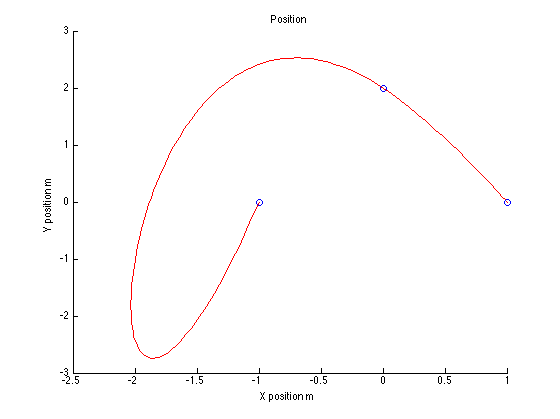
\includegraphics[width =\textwidth]{cubic.png}


b. What is the minimum order polynomial you need to construct a minimum jerk trajectory? Construct this trajectory, write down your solution, and create a plot as in part 
\paragraph{Solution:}
In order to construct a minimum jerk trajectory we need a 5th order polynomial, which should be represented as: 
\paragraph{}
 \begin{displaymath}
   x(t) = \left\{
     \begin{array}{lr}
       $$-1-1*t + 0*t^2 -0.1478t^3  +0.0823t^4 -0.0086t^5$$& : t \leq 5\\
       $$-1100 +1098.0t -439.6t^2 +87.77t^3 -8.71t^4 +0.3431t^5 $$ & : t \geq 5
     \end{array}
   \right.
\end{displaymath} 
\begin{displaymath}
   y(t) = \left\{
     \begin{array}{lr}  
       $$ - 5t +1.988t^3 -0.589t^4 0.047t^5$$& : t \leq 5\\
       $$ 3117 -3122t +1246.8t^2 -247.37t^3 + 24.35t^4 -0.950t^5 $$ & : t \geq 5
     \end{array}
   \right.
\end{displaymath} 
\\
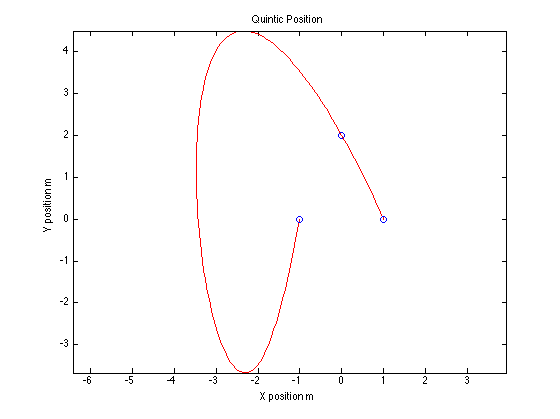
\includegraphics[width = \textwidth]{quintic.png}

c. What is the minimum order polynomial you need to construct a minimum snap trajectory? Construct this trajectory, write down your solution, and create a plot. 
\paragraph{Solution:}
In order to make a minimum snap trajectory it needs at least 7th order polynomial, which can be represented as: 
\paragraph{}
 \begin{displaymath}
   x(t) = \left\{
     \begin{array}{lr}
       $$ -1	-1t 	-0.4105t^4+	0.2334t^5 - 0.04264t^6 +	0.002553t^7 $$& : t \leq 5\\
       $$   12893.2 - 18052.88t	+ 10831.128t^2	- 3610.38t^3 +	721.66t^4 - 	  86.4156t^5+	5.734t^6 - 0.1625t^7 $$ & : t \geq 5
     \end{array}
   \right.
\end{displaymath} 
\begin{displaymath}
   y(t) = \left\{
     \begin{array}{lr}  
       $$-5t +1.804t^4	-0.871t^5	0.144t^6	-0.00807t^7$$& : t \leq 5\\
       $$ -31038.6	+43449.04t	-26072.424t^2+	8690.80t^3	- 1736.357t^4	 + 207.71t^5	- 13.761t^6	+ 0.3892t^7 $$ & : t \geq 5
     \end{array}
   \right.
\end{displaymath} 
\\
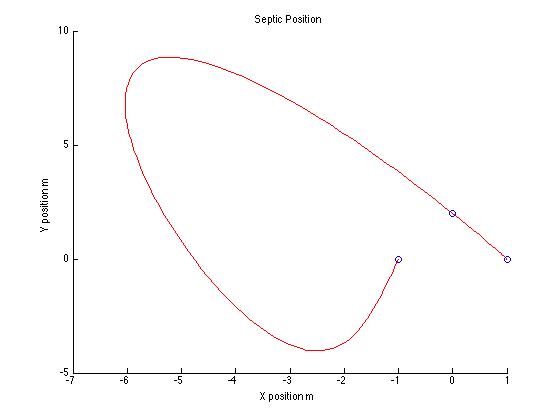
\includegraphics[width = \textwidth]{septic.png}

d. Name one advantage and one disadvantage of choosing a lower order polynomial over a higher one.  
One advantage to using a lower order polynomial is that you have to compute and store less variables, when computing the trajectories. However using a higher order polynomial ensures that your trajectories are smoother the higher the order. 


\paragraph{3.}

Calculate the angular velocities $\omega^s$ and $\omega^b$ for the rotation:
\begin{align}
R = e^{\hat{\omega}_1 t} e^{\hat{\omega}_2 t}
\end{align}

\paragraph{Solution:}
\begin{align}
\hat{\omega}^s  = \dot{R}R^T
\end{align}
\begin{align}
\dot{R} = \hat{\omega}_1e^{\hat{\omega}_1t}e^{\hat{\omega}_2t} + e^{\hat{\omega}_1t}e^{\hat{\omega}_2t}\hat{\omega}_2
\end{align}
$$  \hat{\omega}^s =(\hat{\omega}_1e^{\hat{\omega}_1t}e^{\hat{\omega}_2t} + e^{\hat{\omega}_1t}e^{\hat{\omega}_2t}\hat{\omega}_2)R^T
$$
$$
\hat{\omega}^s =(\hat{\omega}_1R + R\hat{\omega}_2)R^T
$$
$$
\hat{\omega}^s =\hat{\omega}_1 + R\hat{\omega}_2R^T
$$
\begin{align}
\hat{\omega}^b = R^T\dot{R} 
\end{align}
$$
\hat{\omega}^b = R^T( \hat{\omega}_1e^{\hat{\omega}_1t}e^{\hat{\omega}_2t} + e^{\hat{\omega}_1t}e^{\hat{\omega}_2t}\hat{\omega}_2) 
$$

$$
\hat{\omega}^b = R^T(\hat{\omega}_1R  + R\hat{\omega}_2) 
$$
$$
\hat{\omega}^b =  R^T\hat{\omega}_1R  + \hat{\omega}_2 
$$
\paragraph{4.} {
What skew-symmetric matrix $\hat{\omega} \in so(3)$ corresponds to the rotation
\begin{equation*}
R= \begin{bmatrix}
   -0.3038 &  -0.6313 & -0.7135\\
   -0.9332  &  0.3481   & 0.0893\\
    0.1920   & 0.6930 &  -0.6949\\
\end{bmatrix}
\end{equation*}


\paragraph{Solution:}
Rodriguez's formula lets us transform this rotation matrix R into axis angle 
\begin{equation*}
R= I \cos(\phi) + \omega\omega^T(1 - \cos(\phi)) + \hat{\omega}\sin(\phi)
\end{equation*}
\begin{equation}
\tau = (R_{11} + R_{22} + R_{33})
\end{equation}
$$
\phi = \arccos(\frac{\tau -1}{2})
$$
$$
\hat{\omega} =  \frac{1}{2\sin(\phi)}(R - R^T) 
$$
$$
\hat{\omega} = \begin{bmatrix}
         0  &  0.2673 &  -0.8018\\
   -0.2673    &     0 &  -0.5345\\
    0.8018    &0.5345    &     0\\

\end{bmatrix}
$$

Is it unique?
\paragraph{Solution:}
This skew symmetric is not unique, because it is not constrained in the problem statement so this matrix is not unique. 
Reduced row echloen form yields this result:
\begin{equation*}
R= \begin{bmatrix}
   		1  &      0   & 1.9997\\
         0   & 1&  -2.9993\\
         0     &    0     &    0\\
\end{bmatrix}
\end{equation*}
%\bibliography{ref}
%\bibliographystyle{plain}

\end{document}
